\section{信息量的连续性}
\label{sec:info-continuity}

实际使用的概率表往往只是近似：由数据估出，或由另一个模型逼近。两张概率表很接近时，它们的熵、互信息是否也很接近？差多少？在有限字母表上，答案是肯定的，并且可以用总变差给出明确的界；字母表无限或变量连续时，接近的分布可以有相差很远甚至无穷的信息量。

\paragraph{有限字母表上的熵}
设$P,Q$是$m$个元素的集合上的概率分布，记
\[
  \theta=\lVert P-Q\rVert_1=\sum_x\lvert p(x)-q(x)\rvert,
\]
它是总变差$d_{\mathrm{TV}}(P,Q)$的两倍。证明需要一个关于$\psi(t)=-t\ln t$的引理：两个概率值相差不超过$\tfrac12$时，$\psi$的差可以只用这个差值控制。

\begin{lemma}[单项的连续性]
\label{lem:info-psi-continuity}
设$s,t\in[0,1]$，$\lvert s-t\rvert=u\leq\tfrac12$。则$\lvert\psi(s)-\psi(t)\rvert\leq\psi(u)$。
\end{lemma}

\begin{proof}
不妨设$s=t+u$，$t\in[0,1-u]$。令$g(t)=\psi(t+u)-\psi(t)$。$\psi$凹，所以对固定的$u$，增量$g$随$t$递减，$g$的值介于两端点之间：
\[
  g(0)=\psi(u),\qquad g(1-u)=\psi(1)-\psi(1-u)=-\psi(1-u).
\]
因此$\lvert g(t)\rvert\leq\max\{\psi(u),\psi(1-u)\}$。只需再证$u\leq\tfrac12$时$\psi(u)\geq\psi(1-u)$。令$\chi(u)=\psi(u)-\psi(1-u)$，则$\chi(0)=\chi(\tfrac12)=0$，并且在$(0,\tfrac12)$上
\[
  \chi''(u)=-\frac1u+\frac{1}{1-u}<0.
\]
$\chi$在$[0,\tfrac12]$上凹且两端为零，所以$\chi\geq0$。
\end{proof}

\begin{theorem}[熵的连续性]
\label{thm:info-entropy-continuity}
设$P,Q$是$m$个元素的集合上的概率分布，$\theta=\lVert P-Q\rVert_1\leq\tfrac12$。则
\begin{equation}
  \lvert H(P)-H(Q)\rvert\leq\theta\ln\frac{m}{\theta}.
  \label{eq:info-entropy-continuity}
\end{equation}
\end{theorem}

\begin{proof}
记$u_x=\lvert p(x)-q(x)\rvert$，每个$u_x\leq\theta\leq\tfrac12$。$\theta=0$时两边为零，下设$\theta>0$。由三角不等式与引理~\ref{lem:info-psi-continuity}，
\[
  \lvert H(P)-H(Q)\rvert\leq\sum_x\lvert\psi(p(x))-\psi(q(x))\rvert\leq\sum_x\psi(u_x).
\]
把$u_x/\theta$看成一个概率向量（它们的和为$1$），用$\ln u_x=\ln(u_x/\theta)+\ln\theta$拆开，得到
\[
  \sum_x\psi(u_x)=\theta\sum_x\psi\Bigl(\frac{u_x}{\theta}\Bigr)-\theta\ln\theta.
\]
右端的和是一个$m$点分布的熵，由定理~\ref{thm:info-entropy-range}不超过$\ln m$，于是
\[
  \sum_x\psi(u_x)\leq\theta\ln m-\theta\ln\theta=\theta\ln\frac{m}{\theta}.\qedhere
\]
\end{proof}

界中有两个因素。$\theta\ln(1/\theta)$说明熵对分布的依赖不是Lipschitz的：$\theta$很小时，$\theta\ln(1/\theta)$比$\theta$大得多，这对应二元熵函数在端点处的无穷斜率。$\theta\ln m$说明字母表越大，同样的总变差可能造成越大的熵差：一小部分质量可以被分散到很多个取值上。

\begin{BookInlineFigure}
  \centering
  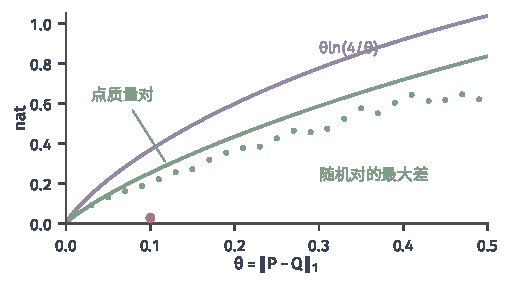
\includegraphics[width=86mm]{figures/07-probability/04-distribution-analysis/matplotlib/info-continuity/figure.pdf}
  \caption{四元字母表上熵差与$\theta=\lVert P-Q\rVert_1$。紫线为界$\theta\ln(4/\theta)$；绿线为点质量$P=(1,0,0,0)$与$Q=(1-\tfrac{\theta}{2},\tfrac{\theta}{6},\tfrac{\theta}{6},\tfrac{\theta}{6})$的熵差；绿点为$200000$对随机分布（种子$1$）在各$\theta$区间内的最大熵差。红点为四字母表与$(0.45,0.3,0.125,0.125)$：$\theta=0.1$，熵差$0.027$。}
  \label{fig:info-continuity}
\end{BookInlineFigure}

图~\ref{fig:info-continuity}比较了界与实际的熵差。离点质量很近的分布熵差最大：把一点质量从确定的结果匀给其余三个值，熵从$0$升到$h_{\mathrm{b}}(\theta/2)+\tfrac{\theta}{2}\ln3$，这条曲线在原点处的斜率同样是无穷大。随机抽取的分布对大多远离这种极端，熵差小得多。四字母表的例子中$\theta=0.1$，界为$0.1\ln40\approx0.369$，实际熵差只有$0.027$：界对最坏情形是合理的，对具体一对分布可能很宽。

\paragraph{有限组合的信息量}
互信息、条件熵在有限字母表上都是几个熵的有限组合，例如$I(X;Y)=H(X)+H(Y)-H(X,Y)$。设$(X,Y)$在$\mathcal{X}\times\mathcal{Y}$上的两个联合分布相差$\theta=\lVert P_{X,Y}-Q_{X,Y}\rVert_1\leq\tfrac12$。边缘分布的$L^{1}$距离不超过联合分布的：
\[
  \sum_x\Bigl\lvert\sum_y\bigl(p(x,y)-q(x,y)\bigr)\Bigr\rvert\leq\sum_{x,y}\lvert p(x,y)-q(x,y)\rvert=\theta.
\]
函数$t\mapsto t\ln(m/t)$在$t\leq m/\mathrm{e}$时递增，所以对边缘也可以用$\theta$代替各自的距离。对三项分别用式~\eqref{eq:info-entropy-continuity}，记$m_X=\lvert\mathcal{X}\rvert$，$m_Y=\lvert\mathcal{Y}\rvert$，得到
\begin{equation}
  \lvert I_P(X;Y)-I_Q(X;Y)\rvert\leq\theta\ln\frac{m_X}{\theta}+\theta\ln\frac{m_Y}{\theta}+\theta\ln\frac{m_Xm_Y}{\theta}.
  \label{eq:info-mi-continuity}
\end{equation}
同样的办法适用于条件熵$H(X\mid Y)=H(X,Y)-H(Y)$和条件互信息。界中的字母表大小来自所用的每一个熵。

\paragraph{无限字母表}
字母表无限时，没有类似的界。取
\[
  P_n=\bigl(1-\tfrac1n\bigr)\delta_0+\tfrac1n\operatorname{Unif}\{1,\dots,K_n\},\qquad K_n=\lceil\mathrm{e}^{n^{2}}\rceil,
\]
它与$\delta_0$的总变差是$\tfrac1n\to0$。设$X\sim P_n$，令$E=\mathbf{1}_{\{X\neq0\}}$。$E$是$X$的函数，由链式法则~\eqref{eq:info-entropy-chain-rule}先揭示$E$再揭示$X$：$E=0$时$X=0$已确定，$E=1$时$X$在$K_n$个值上均匀。于是
\[
  H(P_n)=h_{\mathrm{b}}(\tfrac1n)+\tfrac1n\ln K_n\geq\tfrac1n\cdot n^{2}=n\to\infty,
\]
而$H(\delta_0)=0$。一小份质量被摊到极多的取值上，熵就可以任意大。所以有限字母表上的连续性不能直接推广，需要额外控制质量在远处的分布方式，例如统一的尾部衰减条件。

\paragraph{连续情形与弱收敛}
对密度，弱收敛更不能保证微分熵收敛。在$[0,1]$上取密度
\[
  f_n(x)=1+\sin(2\pi nx),\qquad n=1,2,\dots.
\]
对任意连续函数$\varphi$，$\int_0^1\varphi(x)\sin(2\pi nx)\,\mathrm{d}x\to0$（Riemann–Lebesgue引理），所以$f_n$对应的分布弱收敛于$\operatorname{Unif}(0,1)$，后者的微分熵为$0$。但换元$u=nx$并利用周期性，每个$f_n$的微分熵相同：
\[
  h(f_n)=-\int_0^1(1+\sin2\pi u)\ln(1+\sin2\pi u)\,\mathrm{d}u=\ln2-1\approx-0.307.
\]
振荡越来越快，在任意固定区间上的质量与均匀分布越来越接近，但密度的高低起伏从未减小，微分熵也就停在$\ln2-1$。

\begin{BookInlineFigure}
  \centering
  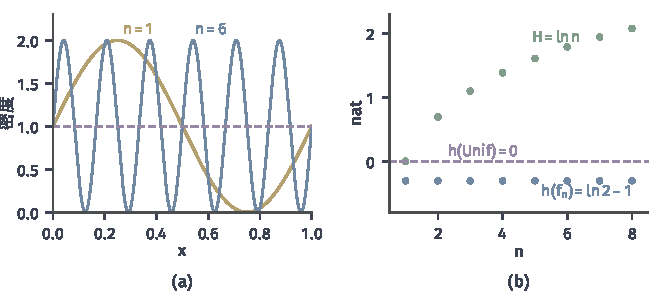
\includegraphics[width=112mm]{figures/07-probability/04-distribution-analysis/matplotlib/info-weak-entropy/figure.pdf}
  \caption{弱收敛不保证熵收敛。(a)密度$f_n(x)=1+\sin(2\pi nx)$，$n=1$（黄）与$n=6$（蓝），紫虚线为极限$\operatorname{Unif}(0,1)$的密度。(b)$h(f_n)$（蓝点，数值积分）恒为$\ln2-1$，极限的微分熵为$0$（紫虚线）；绿点为$\{\tfrac1n,\tfrac2n,\dots,1\}$上均匀分布的熵$\ln n$，它们也弱收敛于$\operatorname{Unif}(0,1)$。单位nat。}
  \label{fig:info-weak-entropy}
\end{BookInlineFigure}

图~\ref{fig:info-weak-entropy}(b)还给出了另一种失效。在$n$个等距点$\tfrac1n,\tfrac2n,\dots,1$上的均匀分布弱收敛于$\operatorname{Unif}(0,1)$，熵是$\ln n\to\infty$，而极限没有概率质量，离散熵无从谈起，只有微分熵$0$。离散分布逼近连续分布时，离散熵按式~\eqref{eq:info-quantized-entropy}的方式发散，要减去$\ln(1/n)$才有有限的极限。

所以在连续空间中谈论信息量的收敛，除了分布本身收敛，还要有关于密度的正则性（如一致有界、等度连续）与尾部的控制。弱收敛只控制有界连续函数的平均，而$-\ln f$既不有界，又随分布本身改变，不在弱收敛能控制的函数之内。
